\section{Глава вторая}
\subsection{Функции, используемые в проекте}
За 9 лет работы над проектом «Час ЕГЭ» была разработан нестандартная библиотека для упрощения многих задач. Далее представлены наиболее используемые функции из неё.

\textbf{Работа с массивами}

\textbf{Многочлены}

Элементы одномерного массива Array --- коэффициенты, стоящие в порядке возрастания степеней.

\texttt{\textcolor{Orange}{Array}.\textcolor{Blue}{prototype}.\textcolor{Purple}{mn\_proizv}=\textcolor{Red}{function}()}

Находит производную от многочлена.

\texttt{\textcolor{Orange}{Array}.\textcolor{Blue}{prototype}.\textcolor{Purple}{mn\_vychisl}=\textcolor{Red}{function}()
}

Находит корни многочлена.

\texttt{
	\textcolor{Orange}{Array}.\textcolor{Blue}{prototype}.\textcolor{Purple}{mn\_txt}=\textcolor{Red}{function}()}

TeX-представление многочлена.%%%???

\texttt{
	\textcolor{Orange}{Array}.\textcolor{Blue}{prototype}.\textcolor{Purple}{mn\_pervoobr}=\textcolor{Red}{function}()
}

Находит первообразную от многочлена.%%TODO в чёр разница то??

\texttt{
	\textcolor{Orange}{Array}.\textcolor{Blue}{prototype}.\textcolor{Purple}{mn\_txtmas}=\textcolor{Red}{function}()
}

TeX-представление многочлена.

\texttt{
	\textcolor{Orange}{Array}.\textcolor{Blue}{prototype}.\textcolor{Purple}{mt\_pryam}=\textcolor{Red}{function}()
}

Возвращает коэффициенты $a$ и $b$ прямой $y=ax+b$, проходящей через две первые точки.

\textbf{Вспомогательные функции для массивов}

\texttt{
	\textcolor{Orange}{Array}.\textcolor{Blue}{prototype}.\textcolor{Purple}{shuffle}=\textcolor{Red}{function}(b)
}

Перемешивает массив случайным образом. Если b, то ещё и рекурсивно на один уровень.

\hypertarget{iz}{\texttt{
		\textcolor{Orange}{Array}.\textcolor{Blue}{prototype}.\textcolor{Purple}{iz}=\textcolor{Red}{function}(p1)
	}}

Если p1 опущено, возвращает случайный элемент массива, иначе последовательность p1 неповторяющихся элементов массива.

\textbf{Матрицы}

\texttt{
	\textcolor{Red}{function} \textcolor{Purple}{multiplyMatrix}(A,B)
}

Умножает матрицу A на B, возвращает результат в матрице C.

\texttt{
	\textcolor{Red}{function} \textcolor{Purple}{Determinant}(A)
}

Возвращает определитель матрицы A.

\texttt{
	\textcolor{Red}{function} \textcolor{Purple}{MatrixCofactor}(i,j,A)
}

Возвращает алгебраическое дополнение матрицы A.

\texttt{
	\textcolor{Red}{function} \textcolor{Purple}{AdjugateMatrix}(A)
}

Возвращает союзную(присоединенную) матрицу.

\texttt{
	\textcolor{Red}{function} \textcolor{Purple}{rang\_mat}(А)
}

Возвращает ранг матрицы A.

\texttt{
	\textcolor{Red}{function} \textcolor{Purple}{InverseMatrix}(B)
}

Возвращает обратную  к B матрицу.

\texttt{
	\textcolor{Red}{function} \textcolor{Purple}{generateMatrix}(stroki,stolbcy,min,max,p1)
}

Генерирует матрицу из случайных чисел.

\textbf{Работа с числами}

\hypertarget{chislitlx}{\texttt{
	\textcolor{Orange}{Number}.\textcolor{Blue}{prototype}.\textcolor{Purple}{chislitlx}=\textcolor{Red}{function}(p1,p2)
}}

Возвращает строку, состоящую из данного числа и подходящего падежа слова p1, при этом
полученное словосочетанию стоит в падеже p2 (если не указан - именительный).

\texttt{
	\textcolor{Orange}{Number}.\textcolor{Blue}{prototype}.\textcolor{Purple}{pow}=\textcolor{Red}{function}(n)
}

Возвращает число в степени n.

\texttt{
	\textcolor{Orange}{Number}.\textcolor{Blue}{prototype}.\textcolor{Purple}{sqrt}=\textcolor{Red}{function}(n)
}

Возвращает квадратный корень из числа.

\texttt{
	\textcolor{Orange}{Number}.\textcolor{Blue}{prototype}.\textcolor{Purple}{sqr}=\textcolor{Red}{function}()
}

Возвращает квадрат числа.

\texttt{
	\textcolor{Orange}{Number}.\textcolor{Blue}{prototype}.\textcolor{Purple}{abs}=\textcolor{Red}{function}()
}

Возвращает модуль числа.

\texttt{
	\textcolor{Orange}{Number}.\textcolor{Blue}{prototype}.\textcolor{Purple}{floor}=\textcolor{Red}{function}()
}

Возвращает число, округленное до целого в меньшую сторону.

\texttt{
	\textcolor{Orange}{Number}.\textcolor{Blue}{prototype}.\textcolor{Purple}{ceil}=\textcolor{Red}{function}()
}

Возвращает число, округленное до целого в большую сторону.

\texttt{
	\textcolor{Orange}{Number}.\textcolor{Blue}{prototype}.\textcolor{Purple}{pm}=\textcolor{Red}{function}()
}

Случайным образом возвращает число или ему противоположное.

\texttt{
	\textcolor{Orange}{Number}.\textcolor{Blue}{prototype}.\textcolor{Purple}{ts}=\textcolor{Red}{function}()
}
%%зачем? и пример
Приводит число к стандартному виду (с десятичной запятой и не более чем 10 знаками после неё).
Необходимо для отсечения лишней точности.

Пример:
\begin{lstlisting}[frame=none]
	let number1=1/33;
	let number2=(1/33).ts()
\end{lstlisting}
\fbox{
	\parbox{10cm}{
		$number1=0.030303030303030304$

		$number2=0,0303030303$
	}}

	\vspace{\baselineskip}
\texttt{
	\textcolor{Orange}{Number}.\textcolor{Blue}{prototype}.\textcolor{Purple}{texfracpi}=\textcolor{Red}{function}(p1)
}

Возвращает TeX-представление дроби, у которой в числителе данное число, умноженное на $\pi$, а в знаменателе p1.
Случай p1=1 учитывается.

\texttt{
	\textcolor{Orange}{Number}.\textcolor{Blue}{prototype}.\textcolor{Purple}{texsqrt}=\textcolor{Red}{function}(p1,p2)
}

TeX-представление корня из данного числа.
Если данное число - полный квадрат, то корень из числа.
Если p1, то из-под корня будут вынесены возможные множители.
Если p1, p2 и из-под корня выносится единица, то она будет опущена.

\texttt{
	\textcolor{Orange}{Number}.\textcolor{Blue}{prototype}.\textcolor{Purple}{isZ}=\textcolor{Red}{function}()
}

Возвращает true, если число n целое.

\texttt{
	\textcolor{Orange}{Number}.\textcolor{Blue}{prototype}.\textcolor{Purple}{isPolnKvadr}=\textcolor{Red}{function}()
}

Возвращает true, если число является полным квадратом.

\textbf{Работа с текстом}

\hypertarget{toZagl}{\texttt{
		\textcolor{Orange}{Number}.\textcolor{Blue}{prototype}.\textcolor{Purple}{toZagl}=\textcolor{Red}{function}()
	}}

Возвращает исходную строку с первой заглавной буквой.

\texttt{
	\textcolor{Orange}{Number}.\textcolor{Blue}{prototype}.\textcolor{Purple}{esli}=\textcolor{Red}{function}()
}

Возвращает данную строку, если p1, и пустую в противном случае.

\texttt{
	\textcolor{Orange}{Number}.\textcolor{Blue}{prototype}.\textcolor{Purple}{plusminus}=\textcolor{Red}{function}()
}

Возвращает упрощенное выражение, вставляя между числами необходимые знаки и убирая нулевые.

\textbf{Работа с canvas}

\texttt{
	\textcolor{Orange}{CanvasRenderingContext2D}.\textcolor{Blue}{prototype}.\textcolor{Purple}{drawLine}=\textcolor{Red}{function}(x1,y1,x2,y2)
}

Рисует линию из точки (x1,y1) в (x2,y2).

\texttt{
	\textcolor{Orange}{CanvasRenderingContext2D}.\textcolor{Blue}{prototype}.\textcolor{Purple}{fillKrug}=\textcolor{Red}{function}(x,y,r)
}

Рисует круг с центром в (x,y) и радиусом r.

\texttt{
	\textcolor{Orange}{CanvasRenderingContext2D}.\textcolor{Blue}{prototype}.\textcolor{Purple}{drawArrow}=\textcolor{Red}{function}(x1, y1, x2, y2, arrowType)
}%%TODO Узнать зачем arrowType

Рисует стрелку из точки (x1,y1) в (x2,y2).

\hypertarget{drawCoordPlane}{\texttt{
		\textcolor{Orange}{CanvasRenderingContext2D}.\textcolor{Blue}{prototype}.\textcolor{Purple}{drawCoordPlane }=\textcolor{Red}{function}(w, h, kl, text, mash)
	}}

Рисует координатную плоскость. w и h  \-- её размеры, kl \-- объект с полями hor и ver(высота и ширина клетки), text \-- объект с полями x1 и y1(единичные отрезки типа string), sh1 и sh2 (шрифты для x1, y1, по умолчанию 12px) и mash - масштаб изображения (по умолчанию равно 1).

\texttt{
	\textcolor{Orange}{CanvasRenderingContext2D}.\textcolor{Blue}{prototype}.\textcolor{Purple}{setkaVer2}=
	\newline
	\textcolor{Red}{function}(h, w, hor, ver, mash)
}

Рисует прямоугольную сетку. w и h  \-- её размеры, hor и ver \-- высота и ширина клетки, mash - масштаб (по умолчанию равно 1).

\hypertarget{graph9AmarkCircles}{\texttt{
		\textcolor{Red}{function} \textcolor{Purple}{graph9AmarkCircles}(ct, XY, maxQuantity, radius)
	}}

Рисует maxQuantity точек в координатах из двумерно массива XY радиусом radius.
%%Переписать!

\hypertarget{graph9AdrawFunction}{\texttt{
		\textcolor{Red}{function} \textcolor{Purple}{graph9AdrawFunction}(ct, f, o)
	}}

Рисует график f(x). Границы отображения задаются объектом o с полями maxX, maxY, minX, minY.

\textbf{Вспомогательные функции}

\hypertarget{sluchch}{\texttt{
		\textcolor{Red}{function} \textcolor{Purple}{sluchch}(n,k,s)
	}}

Возвращает случайное число от n до k с шагом s по умолчанию 1).
Эта функция используется настолько часто, что для неё была придумана сокращённая форма sl().

\hypertarget{slKrome}{\texttt{
		\textcolor{Red}{function} \textcolor{Purple}{slKrome}(a,p1,p2,p3)
	}}

Возвращает случайное число, кроме a. Если a \-- массив, то не содержащееся в нём; Если число или строка, то не равное ему; Если функция, принимающая параметр - то не удовлетворяющее ей.

\texttt{
	\textcolor{Red}{function} \textcolor{Purple}{sluchDel}(a)
}

Случайный делитель числа a.

\texttt{
	\textcolor{Red}{function} \textcolor{Purple}{sluchiz}(a,n)
}

Возвращает массив из n случайных не повторяющихся элементов массива a.

\texttt{
	\textcolor{Red}{function} \textcolor{Purple}{slLetter}(b)
}

Возвращает случайную букву английского алфавита.%%зачем b?

\hypertarget{intPoints}{\texttt{
		\textcolor{Red}{function} \textcolor{Purple}{intPoints}(f,o)
	}}

Возвращает двумерный массив из всех целых точек графика f(x). Границы нахождения точек задаются объектом o с полями maxX, maxY, minX, minY.
\newpage
\subsection{Вклад автора в расширение каталога}
\begin{lstlisting}
(function() {
	'use strict';
	NAinfo.requireApiVersion(0, 2);
	let ves = sluchch(10, 100);
	let pr1, pr2, answ;
	do {
		pr1 = sluchch(4, 20);
		pr2 = sluchch(70, 90);
		answ = (ves * (100 - pr1)) / (100 - pr2);
	} while (!(answ * 100).isZ());
	let pair = sklonlxkand([
		['абрикос', 'курага'],
		['виноград', 'изюм'],
		[
			['финик', 'яблоко', 'груша', 'банан', 'дыня', 'персик',
				'инжир', 'манго', 'папайя', 'хурма', 'ананас', 'кокос',
				'шиповник', 'клюква', 'барбарис', 'клубника', 'вишня'
			].iz(),
			'сухофрукт'
		],
	].iz());
	NAtask.setTask({
		text: 'При сушке ${pair[0].re} получается ${pair[1].ie}.' +
			' Сколько килограммов ${pair[0].re} потребуется для получения 
		${ves} килограммов ${pair[1].re}, ' +
			'если ${pair[0].ie} содержит ${pr2}\% воды, а ${pair[1].ie} 
		содержит ${pr1}\% воды?',
		answers: answ,
	});
})();
//Обзад  109083
		\end{lstlisting}
Примеры генерируемых задач:

\vspace{\baselineskip}
\fbox{%
	\parbox{17cm}{%
		При сушке абрикоса получается курага. Сколько килограммов абрикоса
		потребуется для получения 66 килограммов кураги, если абрикос содержит
		90\% воды, а курага содержит 20\% воды?}%
}
\vspace{\baselineskip}

\fbox{%
	\parbox{17cm}{%
		При сушке дыни получается сухофрукт. Сколько килограммов дыни потребуется
		для получения 73 килограммов сухофрукта, если дыня содержит 88\% воды, а
		сухофрукт содержит 7\% воды?}%
}
\vspace{\baselineskip}

\fbox{%
	\parbox{17cm}{%
		При сушке винограда получается изюм. Сколько килограммов винограда
		потребуется для получения 70 килограммов изюма, если виноград содержит
		81\% воды, а изюм содержит 5\% воды?}%
}
\vspace{\baselineskip}

\begin{lstlisting}
	(function() {
		'use strict';
		NAinfo.requireApiVersion(0, 2);
		let child_1 = sklonlxkand(['Петя', 'Коля', 'Вася', 'Ваня', 'Саша', 'Женя', 'Никита', 'Арсений', 'Антон', 'Яков',
				'Рома', 'Олег', 'Кирилл', 'Данил', 'Даниил', 'Арик', 'Ярик', 'Фома', 'Дима', 'Артём', 'Матвей', 'Максим', 'Игорь'
			].iz()),
			child_2 = ['Алёна', 'Саша', 'Женя', 'Вика', 'Арина', 'Маша', 'Лена', 'Оля', 'Катя', 'Марина', 'Аня', 'Наташа',
				'Ирина', 'Настя', 'Ирма', 'Кристина', 'Ира', 'Мила', 'Тома', 'Любовь3', 'Вера', 'Надежда', 'Снежана',
			].iz(),
			work = sklonlxkand(['работа', 'тест'].iz()),
			nosame = 'одинаковый',
			answ = ['выполнять ', 'решать ', 'делать '].iz();
		let job, doing, kr = '';
		if (work.ie == 'тест') {
			job = sklonlxkand('вопрос');
			doing = 'отвечает';
			answ = 'отвечать на ';
		} else {
			job = sklonlxkand(['задание', 'задача', 'пример', 'номер'].iz());
			kr = ['контрольную', 'проверочную', 'экзаменационную'].iz();
			doing = ['решает', 'делает'].iz();
		}
		let v1 = sluchch(5, 9),
			v2 = v1 + 1,
			razn;
		if (v1 == 7)
			razn = [30, 60].iz();
		else
			razn = sluchch(20, 60, 10);
		if (work.ie == 'работа')
			nosame = 'одинаковую';
		NAtask.setTask({
			text: `${child_1.ie} и ${child_2} выполняют ${nosame}  ${kr.esli(work.ie == 'работа')} ${work.ve}. ${child_2} ` +
				`${doing}   за час  ${"на".esli(work.ie == 'тест')} ${v1} ${job.rm}   ${work.re}, а ${child_1.ie}` +
				`${'на'.esli(work.ie == 'тест ')}  ${v2}.` +
				` Они одновременно начали ${answ} ${job.vm}, ` +
				`и  ${child_2}  закончила  ${work.ve}  позже  ${child_1.re}  на ${razn} ` +
				`минут. Сколько   ${job.rm}   содержит   ${work.ie}?`,
			answers: (razn * v1 * v2) / (60 * (v2 - v1)),
		});
	})();
	//Обзад 99621
\end{lstlisting}
Примеры генерируемых задач:

\vspace{\baselineskip}
\fbox{%
	\parbox{17cm}{%
		Максим и Арина выполняют одинаковую экзаменационную работу. Арина решает
		за час 7 заданий работы, а Максим 8. Они одновременно начали выполнять
		задания, и Арина закончила работу позже Максима на 60 минут. Сколько заданий
		содержит работа?}%
}

\vspace{\baselineskip}
\fbox{%
	\parbox{17cm}{%
		Матвей и Ирма выполняют одинаковую контрольную работу. Ирма решает за час
		9 примеров работы, а Матвей 10. Они одновременно начали решать примеры,
		и Ирма закончила работу позже Матвея на 20 минут. Сколько примеров содержит
		работа?}%
}

\vspace{\baselineskip}
\fbox{%
	\parbox{17cm}{%
		Коля и Женя выполняют одинаковый тест. Женя отвечает за час на 9 вопросов
		теста, а Коля 10. Они одновременно начали отвечать на вопросы, и Женя
		закончила тест позже Коли на 40 минут. Сколько вопросов содержит тест?}%
}
\vspace{\baselineskip}

\begin{lstlisting}
	(function() {
	`use strict`;
	NAinfo.requireApiVersion(0, 2);
	let znam, chisl_1, chisl_2;
	chisl_1 = Math.pow(sluchch(1, 5), 2);
	chisl_2 = chisl_1 * Math.pow(sluchch(1, 10), 2);
	znam = chisl_1 + chisl_2;

	let ugol = om.latbukv.iz();
	let k = sluchch(0, 100);
	let graniz = [
		[`(${k.texfracpi(1)};${(k+0.5).texfracpi(1)})`, 1, 1, `I`],
		[`(${(k+0.5).texfracpi(1)};${(k+1).texfracpi(1)})`, -1, 2, `II`],
		[`(${(k+1).texfracpi(1)};${(k+1.5).texfracpi(1)})`, 1, 3, `III`],
		[`(${(k+1.5).texfracpi(1)};${(k+2).texfracpi(1)})`, -1, 4, `VI`],
	].iz();
	let zn_1, zn_2, zn_3, minus_1 = ``,
		minus_2 = ``,
		grelets = ``;
	switch (sluchch(0, 1)) { 
	case 0:
		zn_1 = `\\tg`;
		zn_2 = `\\cos`;
		zn_3 = `\\sin`;
		if ((graniz[2] == 2) || (graniz[2] == 3)) // cos<0? 
			minus_1 = `-`;
		if ((graniz[2] == 3) || (graniz[2] == 4)) { //sin<0?
			grelets = '<';
			minus_2 = `-`;
		} else
			grelets = `>`;
		break;
	case 1:
		zn_1 = `\\ctg`;
		zn_2 = `\\sin`;
		zn_3 = `\\cos`;
		if ((graniz[2] == 3) || (graniz[2] == 4)) //sin<0?
			minus_1 = `-`;
		if ((graniz[2] == 2) || (graniz[2] == 3)) // cos<0?
		{
			minus_2 = `-`;
			grelets = `<`;
		} else
			grelets = `>`;
		break;
	}
	let answ = graniz[1] * Math.sqrt(chisl_2 / chisl_1);
	grelets = `(Угол ${ugol} принадлежит ${graniz[3]} четверти - $${zn_3}
	{${ugol}}${grelets}0$)`

	NAtask.setTask({
		text: `Найдите $${zn_1}{${ugol}}$, если $${zn_2}{ ${ugol}}=
		${minus_1}\\sqrt{\\frac{${chisl_1}}{${znam}}}$ и $${ugol}\\in 
		${graniz[0]}$.`,
		answers: answ,
		analys: `Найдём $${zn_3}{${ugol}}=\\sqrt{1-(${minus_1}\\sqrt
		\\frac{${chisl_1}}{${znam}}})^{2}=${minus_2}\\sqrt{
			\\frac{${chisl_2}}{${znam}}}$${grelets}.` +
			` Тогда $${zn_1}{${ugol}}=${` - `.esli(!graniz[2]%2)}
			\\sqrt{\\frac{${chisl_2}}{${chisl_1}}}=${answ}$`,

	});
})();
//Обзад  26775
\end{lstlisting}
Примеры генерируемых задач:

\vspace{\baselineskip}
\fbox{%
	\parbox{17cm}{%
		Найдите $\ctg H$, если $\sin H=-\sqrt{\frac{9}{738}}$ и $H\in(37π;75π2)$.

		Найдём $\cos H\sqrt{1-(-\sqrt{\frac{9}{738}})^2=-\sqrt{\frac{729}{738}}}$(Угол H принадлежит
		III четверти - $\cos H<0$). Тогда $\ctg H=\sqrt{\frac{729}{9}}=9$}
}

\vspace{\baselineskip}
\fbox{%
	\parbox{17cm}{%
		Найдите $\tg M$, если $\cos M=\sqrt{\frac{4}{260}}$ и $M\in(\frac{101}{2}π;51π)$.

		Найдём $\sin M=\sqrt{1-(-\sqrt{\frac{9}{738}})^2=-\sqrt{\frac{729}{738}}}$(Угол  M принадлежит
		VI четверти - $sin M<0$). Тогда $\tg  M=\sqrt{\frac{256}{4}}=-8$}
}

\vspace{\baselineskip}
\fbox{%
	\parbox{17cm}{%
		Найдите $\tg Q$, если $\cos Q=-\sqrt{\frac{9}{153}}$ и $Q\in(\frac{171}{2}π;86π)$.

		Найдём $\sin = Q\sqrt{1-(-\sqrt{\frac{9}{153}})^2=\sqrt{\frac{144}{153}}}$(Угол  Q принадлежит
		VI четверти - $sin Q>0$). Тогда $\tg  Q=\sqrt{\frac{144}{9}}=-4$}
}
\vspace{\baselineskip}

\begin{lstlisting}
	(function() {
	'use strict';
	NAinfo.requireApiVersion(0, 2);
	let answ=sluchch(-100,100,0.5);
	let ugol_1=sluchch(1,90);
	let ugol_2=ugol_1.pm()+90*sluchch(1,11,2);
	ugol_1 += 90*sluchch(0,6,2);
	let k_1=sluchch(0,1);
	let k_2 = 1 - k_1;

	let zn=['\\tg','\\ctg'];
	
	NAtask.setTask({
		text: `Найдите значение выражения $${answ}${zn[k_1]}{${ugol_1}^\\circ} \\cdot ${zn[k_1]}{${ugol_2}^\\circ} $.`,
		answers: answ, 
		analys: `По формуле приведения $${zn[k_1]} ${ugol_2}^\\circ=${zn[k_1]}{(${ugol_1+ugol_2}^\\circ-${ugol_2}^\\circ)}=${zn[k_2]}
		{${ugol_1}^\\circ}$.`+
		` Тогда $ ${answ}${zn[k_1]}{${ugol_1}^\\circ} \\cdot${zn[k_2]}{${ugol_1}^\\circ}=${answ}$`,
	});
})();
//Обзад  26771 26770
\end{lstlisting}
Примеры генерируемых задач:

\vspace{\baselineskip}
\fbox{%
	\parbox{17cm}{%
		Найдите значение выражения $-72\tg201^{\circ}\cdot\tg249^{\circ}$.

		По формуле приведения $\tg249^{\circ}=\tg(450^{\circ}-249^{\circ})=\ctg201^{\circ}$.
		Тогда $-72\tg 201^{\circ}\cdot\ctg 201^{\circ}=-72$}}

\vspace{\baselineskip}
\fbox{%
\parbox{17cm}{%
Найдите значение выражения $-58\tg400^{\circ}\cdot \tg410^{\circ}$.

По формуле приведения $\tg410^{\circ}=\tg(810^{\circ}-410^{\circ})=\ctg400^{\circ}$.
Тогда $-58tg400^{\circ}\cdot\ctg400^{\circ}=-58$}}

\vspace{\baselineskip}
\fbox{%
	\parbox{17cm}{%
		Найдите значение выражения $-32\ctg195^{\circ}\cdot\ctg285^{\circ}.$

		По формуле приведения $\ctg285^{\circ}=\ctg(480^{\circ}-285^{\circ})=\tg195^{\circ}$.
		Тогда $-32\ctg195^{\circ}\cdot\tg195^{\circ}=-32$}}
\vspace{\baselineskip}

\begin{lstlisting}
	(function() {
	'use strict';
	NAinfo.requireApiVersion(0, 0);
	let kol = [[4,'четырёх'],[5, `пяти`],[8, `восьми`]].iz();
	let chislo=kol.pop();
	let k = sluchch(1, kol-1);
	let person1 = [`Петя`, `Коля`, `Вася`, `Ваня`, `Никита`, `Арсений`, `Антон`, `Яков`,
		`Рома`, `Олег`, `Кирилл`, `Данил`, `Даниил`, `Арик`, `Ярик`, `Фома`, `Дима`, `Артём`, `Матвей`, `Максим`, `Игорь`,
	].iz(k);
	let person2 = [`Алёна`, `Вика`, `Арина`, `Маша`, `Лена`, `Оля`, `Катя`, `Марина`, `Аня`, `Наташа`,
		`Ирина`, `Настя`, `Ирма`, `Кристина`, `Ира`, `Мила`, `Тома`, `Любовь`, `Вера`, `Надежда`, `Снежана`,
	].iz(kol - k);
	let persons = person1.concat(person2).shuffle();
	let uslov = [`${persons.iz()}`, `девочка`, `мальчик`, ].iz();
	let must = `должен`;
	if (person2.includes(uslov) || uslov == `девочка`)
		must = `должна`;
	let answ;
	switch (uslov) {
	case (`мальчик`):
		answ = k / kol;
		break;
	case (`девочка`):
		answ = (kol - k) / kol;
		break;
	default:
		answ = 1 / kol;
		break;
	}
	if (sl1()) {
		uslov = `не ` + uslov;
		answ = 1 - answ;
	}
	let children = ``;
	for (let i = 0; i < kol - 1; i++) {
		children += persons[i];
		if (i != kol - 2)
			children += `, `;
		else
			children += ` `;
	}
	children += `и ` + persons[kol - 1];
	NAtask.setTask({
		text: `${children} бросили жребий - кому начинать игру. Найдите вероятность того, что начинать игру ${must} будет ${uslov}.`,
		answers: answ,
		analys: `Жребий начать игру может выпасть каждому из ${chislo} детей. Вероятность того, что это будет ${uslov}, равна ${answ}.`,
	});

})();
// 320169,320335,320343
\end{lstlisting}
Примеры генерируемых задач:

\vspace{\baselineskip}
\fbox{%
	\parbox{17cm}{%
		Марина, Вика, Коля, Даниил, Арик, Надежда, Снежана и Наташа бросили жребий - кому начинать игру. Найдите вероятность того, что начинать игру должен будет мальчик.

		Жребий начать игру может выпасть каждому из восьми детей. Вероятность того, что это будет мальчик, равна 0.375.
	}}

\vspace{\baselineskip}
\fbox{%
	\parbox{17cm}{%
		Антон, Олег, Ира, Артём и Коля бросили жребий - кому начинать игру. Найдите вероятность того, что начинать игру должна будет не девочка.

		Жребий начать игру может выпасть каждому из пяти детей. Вероятность того, что это будет не девочка, равна 0.8.
	}}

\vspace{\baselineskip}
\fbox{%
	\parbox{17cm}{%
		Артём, Ирма, Данил, Антон и Максим бросили жребий - кому начинать игру. Найдите вероятность того, что начинать игру должна будет Ирма.

		Жребий начать игру может выпасть каждому из пяти детей. Вероятность того, что это будет Ирма, равна 0.2.
	}}

\vspace{\baselineskip}

\begin{lstlisting}
	(function() {
		'use strict';
		NAinfo.requireApiVersion(0, 0); 
		let ill = sklonlxkand([`гепатит`, `криворучие`, `соннис`, `забыватикус`, `переленеус`, `шоколадодифицит`, `антилогизм`,
			`диабет`, `Ёжико-вирус`, `перфектолиз`, `трудоголизм`, `хладоручие`, `жмотство`, `физико-зависимость`,
			`Фентезикоз`,
		]).iz();
		let persons = sklonlxkand([`физик`, `химик`, `школьник`, `чудик`, `чиновник`, `президент`, `пациент`, `студент`,
			`математик`,
		]).iz();
		let realRez, lozhRez, realIll, answ, prAnsw1, prAnsw2;
		do {
			realRez = sluchch(30, 95);
			lozhRez = sluchch(2, 10);
			realIll = sluchch(1, 95);
			prAnsw1 = (realRez * realIll) / 10000;
			prAnsw2 = (lozhRez * (100 - realIll)) / 10000;
			answ = (realRez * realIll + lozhRez * (100 - realIll)) / 10000;
		} while (!(answ * 10000.0).isZ());
		let Rez;
		if (sl1())
			Rez = `положительным`;
		else {
			Rez = `отрицательным`;
			answ = 1 - answ;
		}
		let veroyt = [`с вероятностью `, `в `];
		if (sl1())
			realRez /= 100;
		if (sl1())
			lozhRez /= 100;
		if (sl1())
			realIll /= 100;
	
		let find = [`вероятность`, `процент`];
		if (sl1())
			find.pop();
		else {
			find.shift();
			answ *= 100;
		}
		NAtask.setTask({
			text: `	Всем ${persons.dm} с подозрением на ${ill.ve} делают анализ крови. ` +
				`Если анализ выявляет ${ill.ve}, то результат анализа называется положительным. ` +
				`У больных ${ill.te} ${persons.rm} анализ даёт положительный результат ${veroyt[0].esli(realRez<1)} ${veroyt[1].esli(realRez>1)} ${realRez.ts()}${`\%`.esli(realRez>1)}. ` +
				`Если ${persons.im} не болен ${ill.te}, то анализ может дать ложный положительный результат ${veroyt[0].esli(lozhRez<1)} ${veroyt[1].esli(lozhRez>1)} ${lozhRez.ts()}${`\%`.esli(lozhRez>1)}. ` +
				`Известно, что ${realIll.ts()}${`\%`.esli(realIll>1)} ${persons.rm}, поступающих с подозрением на ${ill.ve}, действительно больны ${ill.te}. ` +
				`Найдите ${find} того, что результат анализа у ${persons.rm}, поступившего в клинику с подозрением на ${ill.ve}, будет ${Rez}.`,
			answers: answ,
			analys: `Анализ ${persons.rm} может быть положительным по двум причинам:` +
				` 1) ${persons.ie} болеет ${ill.te}, его анализ верен; 2) пациент не болеет ${ill.te}, его анализ ложен.`+
			` По формуле условной вероятности: $${realRez.ts()}${`/100`.esli(realRez>1)}\\cdot${realIll.ts()}${`/100`.esli(realIll>1)} = ${prAnsw1.ts()}$`+
			` и $${lozhRez.ts()}${`/100`.esli(lozhRez>1)}\\cdot(1-${realIll.ts()}${`/100`.esli(realIll>1)}) = ${prAnsw2.ts()}$. ` +
			`События быть больным или быть здоровым образуют полную группу (они несовместны и одно из них непременно наступает),` +
			` поэтому можно применить формулу полной вероятности. Тогда $${prAnsw1.ts()}+${prAnsw2.ts()}=${(prAnsw1+prAnsw2).ts()}$. `+
			`${`Необходимо найти, что анализ будет отрицательным: $1-${(prAnsw1+prAnsw2).ts()}$. `.esli(Rez == `отрицательным`)} `+
			`${`Так как нужно найти процент, умножим полученный ответ на 100: $${(prAnsw1+prAnsw2).ts()}\\cdot100=${answ.ts()}$`.esli(find==`процент`)} `+
			`Ответ: $${answ.ts()}$`,
		});
	
	})();
	//  320207
\end{lstlisting}
Примеры генерируемых задач:

\vspace{\baselineskip}
\fbox{
	\parbox{17cm}{
		Всем школьникам с подозрением на жмотство делают анализ крови. Если анализ
		выявляет жмотство, то результат анализа называется положительным. У больных
		жмотством школьников анализ даёт положительный результат в 66\%. Если школьники
		не болен жмотством, то анализ может дать ложный положительный результат с
		вероятностью 0,09. Известно, что 0,4 школьников, поступающих с подозрением на
		жмотство, действительно больны жмотством. Найдите вероятность того, что
		результат анализа у школьников, поступившего в клинику с подозрением на
		жмотство, будет положительным.

		Анализ школьников может быть положительным по двум причинам: 1) школьник
		болеет жмотством, его анализ верен; 2) пациент не болеет жмотством, его
		анализ ложен. По формуле условной вероятности: $66/100\cdot0,4=0,264$ и
		$0,09\cdot(1-0,4)=0,054$. События быть больным или быть здоровым образуют
		полную группу (они несовместны и одно из них непременно наступает), поэтому
		можно применить формулу полной вероятности. Тогда $0,264+0,054=0,318$. Ответ: $0,318$
	}}

\vspace{\baselineskip}
\fbox{
	\parbox{17cm}{
		Всем чиновникам с подозрением на диабет делают анализ крови. Если анализ
		выявляет диабет, то результат анализа называется положительным. У больных
		диабетом чиновников анализ даёт положительный результат с вероятностью 0,67.
		Если чиновники не болен диабетом, то анализ может дать ложный положительный
		результат в 9\%. Известно, что 73\% чиновников, поступающих с подозрением на
		диабет, действительно больны диабетом. Найдите процент того, что результат
		анализа у чиновников, поступившего в клинику с подозрением на диабет, будет отрицательным.

		Анализ чиновников может быть положительным по двум причинам: 1) чиновник
		болеет диабетом, его анализ верен; 2) пациент не болеет диабетом, его анализ
		ложен. По формуле условной вероятности: $0,67\cdot73/100=0,4891$ и
		$9/100\cdot(1-73/100)=0,0243$. События быть больным или быть здоровым
		образуют полную группу (они несовместны и одно из них непременно наступает),
		поэтому можно применить формулу полной вероятности. Тогда $0,4891+0,0243=0,5134$.
		Необходимо найти, что анализ будет отрицательным: $1-0,5134$. Так как нужно
		найти процент, умножим полученный ответ на 100: $0,5134\cdot100=48,66$ Ответ: $48,66$
	}}

\vspace{\baselineskip}
\fbox{
	\parbox{17cm}{
		Всем школьникам с подозрением на перфектолиз делают анализ крови. Если анализ
		выявляет перфектолиз, то результат анализа называется положительным.
		У больных перфектолизом школьников анализ даёт положительный результат в 91\%.
		Если школьники не болен перфектолизом, то анализ может дать ложный положительный
		результат с вероятностью $0,09$. Известно, что 0,47 школьников, поступающих с
		подозрением на перфектолиз, действительно больны перфектолизом. Найдите процент
		того, что результат анализа у школьников, поступившего в клинику с подозрением
		на перфектолиз, будет отрицательным.

		Анализ школьников может быть положительным по двум причинам: 1) школьник болеет
		перфектолизом, его анализ верен; 2) пациент не болеет перфектолизом, его анализ
		ложен. По формуле условной вероятности: $91/100\cdot0,47=0,4277$ и
		$0,09\cdot(1-0,47)=0,0477$. События быть больным или быть здоровым образуют
		полную группу (они несовместны и одно из них непременно наступает),
		поэтому можно применить формулу полной вероятности. Тогда 0,4277+0,0477=0,4754.
		Необходимо найти, что анализ будет отрицательным: $1-0,4754$. Так как нужно найти
		процент, умножим полученный ответ на 100: $0,4754\cdot100=52,46$ Ответ: $52,46$
	}}

\vspace{\baselineskip}

\begin{lstlisting}
	retryWhileUndefined(function() {
		NAinfo.requireApiVersion(0, 2);
	
		function fp(x) {
			return k * x + d;
		}
	
		function fs(x) {
			return a * (x + b).sqrt() + c;
		}
	
		let x1 = sluchch(1, 6).pm();
		let x2 = sluchch(8, 20);
		let y1 = sl(-6, 6);
		let y2 = sl(0, 20).pm();
		let k = (y1 - y2) / (x1 - x2);
		if (!(k * 1000).isZ() || !k)
			return;
		let d = y1 - k * x1;
		let b = slKrome([-x1, -x2].iz(), -6, 6, 0.5);
		let a = (y1 - y2) / ((x1 + b).sqrt() - (x2 + b).sqrt());
		if (!(a * 1000).isZ())
			return;
		let c = y1 - a * (x1 + b).sqrt();
		let pointss = intPoints(fs, {
			minX: -5,
			maxX: 5,
			minY: -5.5,
			maxY: 5.5,
			step: 1,
		});
		if (pointss.length < 3)
			return;
		let pointsp = intPoints(fp, {
			minX: -5,
			maxX: 5,
			minY: -5.5,
			maxY: 5.5,
			step: 1,
		});
		if (pointsp.length < 2)
			return;
		let find, answ;
		if (sl1()) {
			answ = x2;
			find = 'абсциссу';
		} else {
			answ = y2;
			find = 'ординату';
		}
		let paint1 = function(ct) {
			let h = 300;
			let w = 300;
			//Оси координат
			ct.drawCoordPlane(w, h, {
				hor: 1,
				ver: 1
			}, {
				x1: '1',
				y1: '1',
				sh1: 13,
			}, 20);
			//График
			ct.scale(20, -20);
			ct.lineWidth = 0.1;
			graph9AdrawFunction(ct, fs, {
				minX: -6.5,
				maxX: 7,
				minY: -7,
				maxY: 6,
				step: 0.0005,
			});
			graph9AdrawFunction(ct, fp, {
				minX: -6.5,
				maxX: 7,
				minY: -7,
				maxY: 6,
				step: 0.05,
			});
			//точки
			graph9AmarkCircles(ct, pointss, 3, 0.15);
			graph9AmarkCircles(ct, pointsp, 2, 0.15);
			graph9AmarkCircles(ct, [
				[x1, y1]
			], 2, 0.15);
			//буква
			ct.fillStyle = "blue";
			ct.font = "18px liberation_sans";
			ct.scale(1 / 20, -1 / 20);
			ct.fillText('A', 20 * x1 - 10, -20 * y1 - 10);
		};
		NAtask.setTask({
			text: 'На рисунке изображены графики функций $f(x)=a\\sqrt{x' + ['+', '-'].iz() + 'b}+c$ и $g(x)=kx' + ['+', '-']
				.iz() +
				'd$,' +
				' которые пересекаются в точках $A$ и $B$. Найдите ' + find + ' точки $B$.',
			answers: answ,
			analys: '$f(x)=' + (a + '\\sqrt{x+' + b + '}+' + c + '$').plusminus() + '<br>' +
				'$g(x)=' + (k.ts() + 'x+' + d.ts()).plusminus() + '$<br>' +
				'$A(' + x1 + ';' + y1 + ')$<br>' +
				'$B(' + x2 + ';' + y2 + ')$',
		});
		chas2.task.modifiers.addCanvasIllustration({
			width: 300,
			height: 300,
			paint: paint1,
		});
		return true;
	}, 100000);
	//50927103
	\end{lstlisting}
\newpage
Примеры генерируемых задач:

\begin{figure}[h]
	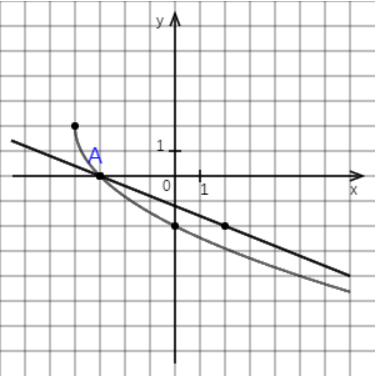
\includegraphics[width=0.4\textwidth]{1.PNG}
\end{figure}
\fbox{
	\parbox{17cm}{
		На рисунке изображены графики функций $f(x)=a\sqrt{x-b}+c$ и
		$g(x)=kx+d$, которые пересекаются в точках A и B. Найдите абсциссу точки B.

		$f(x)=-2\sqrt{x+4}+2$

		$g(x)=-0,4x-1,2$

		$A(-3;0)$

		$B(12;-6)$
	}}

\vspace{\baselineskip}
\begin{figure}[h]
	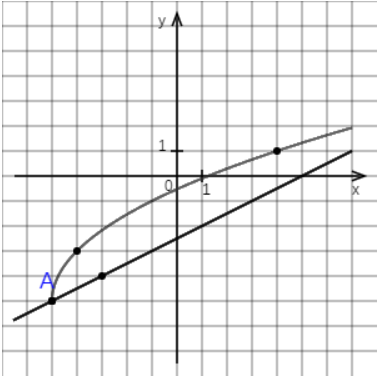
\includegraphics[width=0.4\textwidth]{2.PNG}
\end{figure}
\fbox{
	\parbox{17cm}{
		На рисунке изображены графики функций $f(x)=a\sqrt{x-b}+c$ и $g(x)=kx-d$, 
		которые пересекаются в точках A и B. Найдите абсциссу точки B.
		
		$f(x)=2\sqrt{x+5}-5$

		$g(x)=0,5x-2,5$
		
		$A(-5;-5)$

		$B(11;3)$
		}}

\vspace{\baselineskip}
\begin{figure}[h]
	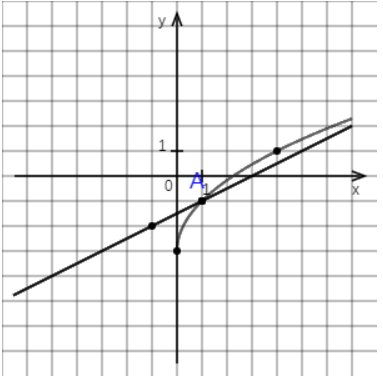
\includegraphics[width=0.4\textwidth]{3.PNG}
\end{figure}
\fbox{
	\parbox{17cm}{На рисунке изображены графики функций $f(x)=a\sqrt{x-b}+c$ и $g(x)=kx-d$,
	 которые пересекаются в точках A и B. Найдите ординату точки B.
	 
	 $f(x)=2\sqrt{x+0}-3$

	 $g(x)=0,5x-1,5$

	 $A(1;-1)$

	 $B(9;3)$
	 }}
%%%%%%%%%%%%%%%%%%%%%

\vspace{\baselineskip}

\begin{lstlisting}
	retryWhileUndefined(function () {
		NAinfo.requireApiVersion(0, 2);
	
		function variant(a, b, x) {
			switch (trigfuncs) {
				case 'sin':
					return a * Math.sin(x * Math.PI / 2) + b;
				case 'cos':
					return a * Math.cos(x * Math.PI / 2) + b;
				case 'tg':
					return a * Math.tan(x * Math.PI / 2) + b;
				case 'ctg':
					return a * (1 / Math.tan(x * Math.PI / 2)) + b;
			}
		}
	
		function f(x) {
			return 0.5 * variant(a, b, x);
		}
		let trigfuncs = ['sin', 'cos', 'tg', 'ctg'].iz();
		let a = sluchch(1, 6).pm();
		let b = sluchch(0, a).pm();
		let find, answ;
		if (sl1() && trigfuncs != 'tg' && trigfuncs != 'ctg') {
			find = 'a';
			answ = a;
		} else {
			find = 'b';
			answ = b;
		}
		let X = [],
			Y = [];
		for (let i = -2; i < 4; i++)
			if (2 * f(i) < 5 && 2 * f(i) > -6) {
				X.push(i);
				Y.push(f(i));
			}
		if (X.length < 2)
			return;
		let paint1 = function (ct) {
			let h = 300;
			let w = 300;
			//Оси координат
			ct.drawCoordPlane(w, h, {
				hor: 2,
				ver: 1
			}, {
				x1: 'π/2',
				y1: '1',
				sh1: 13,
			}, 20);
			//График
			ct.scale(40, -40);
			ct.lineWidth = 0.05;
			graph9AdrawFunction(ct, f, {
				minX: -2.6,
				maxX: 4,
				minY: -4,
				maxY: 3,
				step: 0.05,
			});
			//точки
			graph9AmarkCircles(ct, [X, Y].T(), 2, 0.1);
		};
		NAtask.setTask({
			text: 'На рисунке изображён график функции $f(x)=a\\' + trigfuncs + ' x+b$. Найдите $' + find + '$.',
			answers: answ,
			analys: '$f(x)=' + (a + '\\' + trigfuncs + ' x+' + b).replace('+0', '').plusminus() + '$',
		});
		chas2.task.modifiers.addCanvasIllustration({
			width: 300,
			height: 300,
			paint: paint1,
		});
		return true;
	}, 100000);
	//509123 509130 509137 509143 509287 509295
\end{lstlisting}
\newpage
Примеры генерируемых задач:

\begin{figure}[h]
	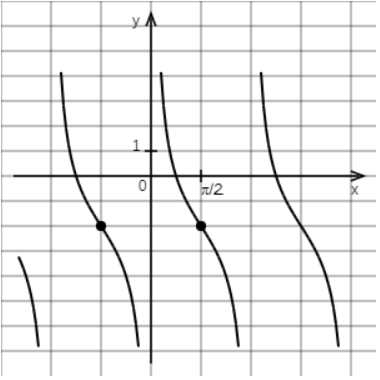
\includegraphics[width=0.4\textwidth]{4.PNG}
\end{figure}
\fbox{
	\parbox{17cm}{
		На рисунке изображён график функции $f(x)=a\ctg x+b$. Найдите $b$.

		$f(x)=2\ctg x-2$
	}}

\vspace{\baselineskip}
\begin{figure}[h]
	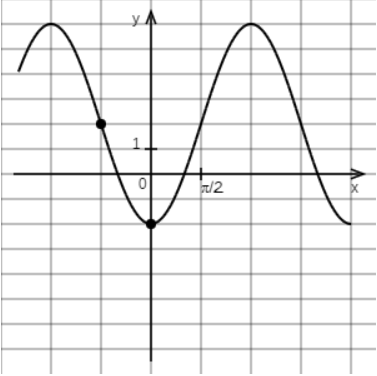
\includegraphics[width=0.4\textwidth]{5.PNG}
\end{figure}
\fbox{
	\parbox{17cm}{
		На рисунке изображён график функции $f(x)=a\cos x+b$. Найдите $a$.

		$f(x)=-4\cos x+2$
	}}

\vspace{\baselineskip}
\newpage
\begin{figure}[h]
	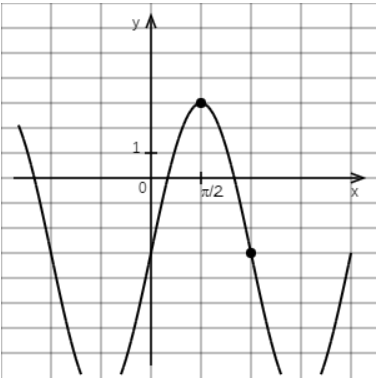
\includegraphics[width=0.4\textwidth]{6.PNG}
\end{figure}
\fbox{
	\parbox{17cm}{
		На рисунке изображён график функции $f(x)=a\sin x+b$. Найдите $b$.
		$f(x)=6\sin x-3$
	}}